% === SUPPORTING INFORMATION ===
%
% Per Stephan: the CRLB derivation is short enough to remain in an Appendix
% in the main document; the supplementary figures (NUTS convergence on
% simulated data and the robustness sweep) live in a separate Supporting
% Information document.

\section*{Appendix: Cram\'er-Rao Scaling of Bin Spacing}

Consider a simplified two-component model in which the normalized signal at
b-value $b$ is
%
\begin{equation*}
  \frac{S(b)}{S_0} = p\,e^{-bD} + (1-p)\,e^{-b(D+\Delta D)},
\end{equation*}
%
with additive Gaussian noise of standard deviation $\sigma$.
The Fisher information for the fraction parameter $p$ is
%
\begin{equation*}
  I(p) = \frac{1}{\sigma^2}\sum_{i=1}^{M}\left(e^{-b_i D} - e^{-b_i(D+\Delta D)}\right)^2.
\end{equation*}
%
Approximating the sum by an integral over $[0,\,b_{\max}]$, expanding the
square, and evaluating in the regime $b_{\max} D \gg 1$ (so that the
exponential boundary terms vanish):
%
\begin{equation*}
  I(p) \propto \frac{1}{2D} - \frac{2}{2D + \Delta D} + \frac{1}{2(D + \Delta D)}.
\end{equation*}
%
For $\Delta D \ll D$, a Taylor expansion yields
$I(p) \propto (\Delta D)^2 / (4D^3)$.
Setting $I = \text{const}$ (equal estimation precision for all bin pairs)
gives $\Delta D \propto D^{3/2}$, Equation~\ref{eq:spacing_scaling} in the
main text.
The same scaling is obtained from the full two-parameter model ($p$ and
$q = 1-p$ independent) via inversion of the $2 \times 2$ Fisher matrix.
This argument is intentionally restricted to the two-compartment limit; the
full multi-compartment problem is treated numerically in the main text.

% --- Supplementary atlas: individual estimated spectra for every ROI ---
% Multi-page atlas embedded with \includepdf.
% REQUIRES \usepackage{pdfpages} in the main preamble.
% Fallback if pdfpages is unavailable: include pages individually with
%   \includegraphics[page=<n>]{figures/figS1_all_roi_spectra.pdf}  (n = 1..20).
\clearpage
\noindent\textbf{Supplementary Atlas: individual estimated spectra for all
149 ROIs.}
Each panel shows one ROI's full NUTS posterior over the eight-bin diffusivity
spectrum ($D = 0.25,\,0.5,\,0.75,\,1.0,\,1.5,\,2.0,\,3.0,\,20\;\umsmm$, left to
right) as box plots: the box spans the interquartile range, the solid line is
the posterior median, the dashed line the posterior mean, and the whiskers the
5th--95th percentiles (fliers suppressed, as the per-bin posteriors are
continuous and unimodal). Each box face is coloured by the within-ROI per-bin
coefficient of variation (CV $=$ posterior std $/$ posterior mean; colorblind-safe
sequential colour plus hatching, light/clean $=$ well identified to
dark/cross-hatched $=$ poorly identified, the same scheme as
Figure~\ref{fig:sensitivity}): the box
\emph{width} is the absolute posterior spread while the colour is the
\emph{relative} spread, so a low-mass outer bin can show a narrow box yet a dark
(relatively uncertain) colour. The green $\times$ marks the tuned-MAP
($\lambda = 10^{-3}$) point estimate. Panels are grouped by anatomical zone and
tissue type (page headers) and ordered by ADC within each group; panel titles
give the patient identifier (the key into the publicly released signal-decay
data), the zone and tissue, and, for tumour ROIs, the biopsy Gleason score and
Grade Group. A companion key file (\texttt{figS1\_roi\_key.csv}) lists the exact
anatomical region and SNR for each panel.
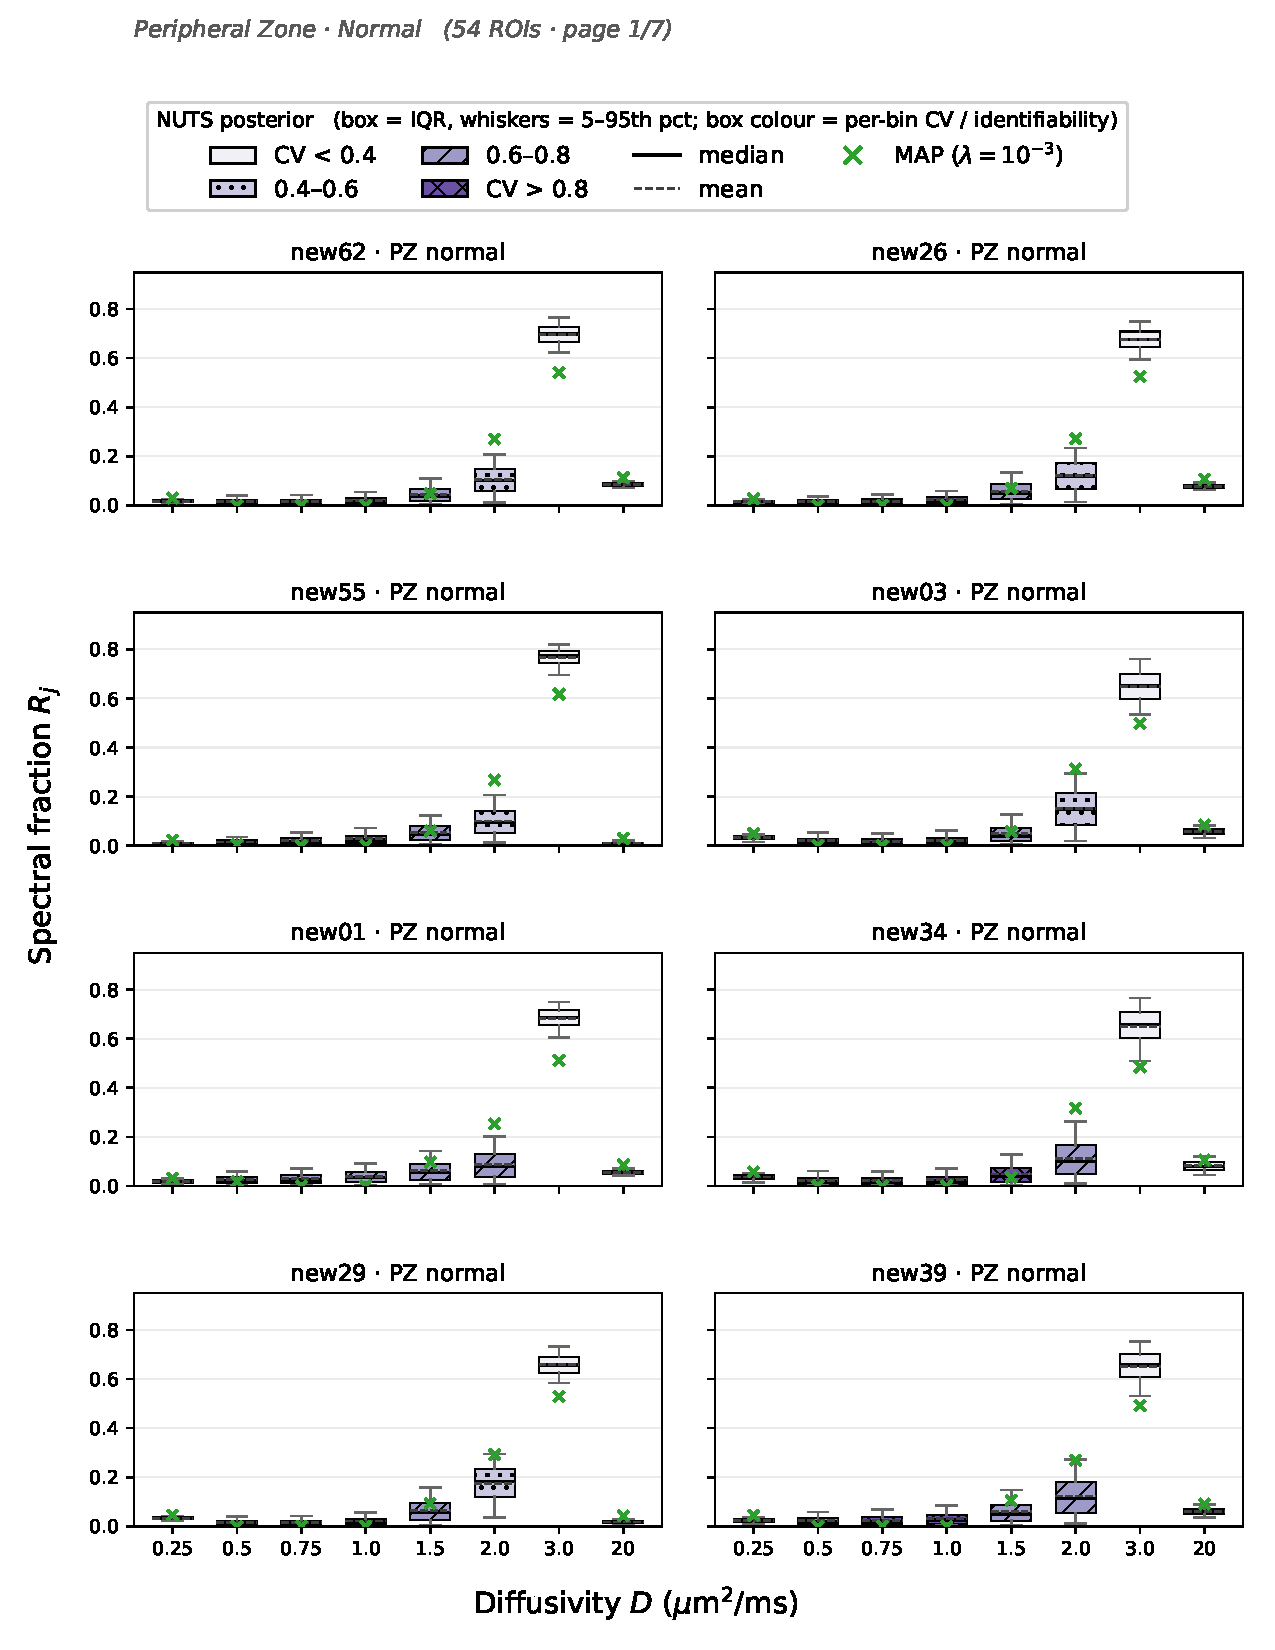
\includepdf[pages=-]{figures/figS1_all_roi_spectra.pdf}

% --- REMOVED 2026-06-02 ---
% Fig S1 (NUTS multi-chain trace plots, fig_trace_simulation.pdf): dropped --
% unreadable and uninformative to readers; convergence is reported in Methods
% (split-Rhat < 1.05 for all 149 ROIs).
% Fig S2 (robustness across spectral shapes, fig_robustness.png): dropped --
% redundant with the recovery panels of main Figure~\ref{fig:validation}, and
% carried unresolved font/colour TODOs. A broader simulation recovery battery
% can be added back to the SI later if desired.

% --- Fig S: Fisher Information Analysis (relocated from the main text 2026-06-01;
%     keeps \label{fig:fisher} so the in-text references in theory/results/discussion
%     resolve to this supplementary figure). ---
\begin{figure}[p]
\centering
% TODO(figure-regen): larger fonts (~+50%); in panel (b) move the legend to
% a free area in the middle of the plot so that it does not cover the bars
% or the improvement-factor labels. NOTE: panel (b) SNR is hard-coded at 150;
% should be regenerated at the cohort-median SNR=303 (see PROJECT_STATE F10).
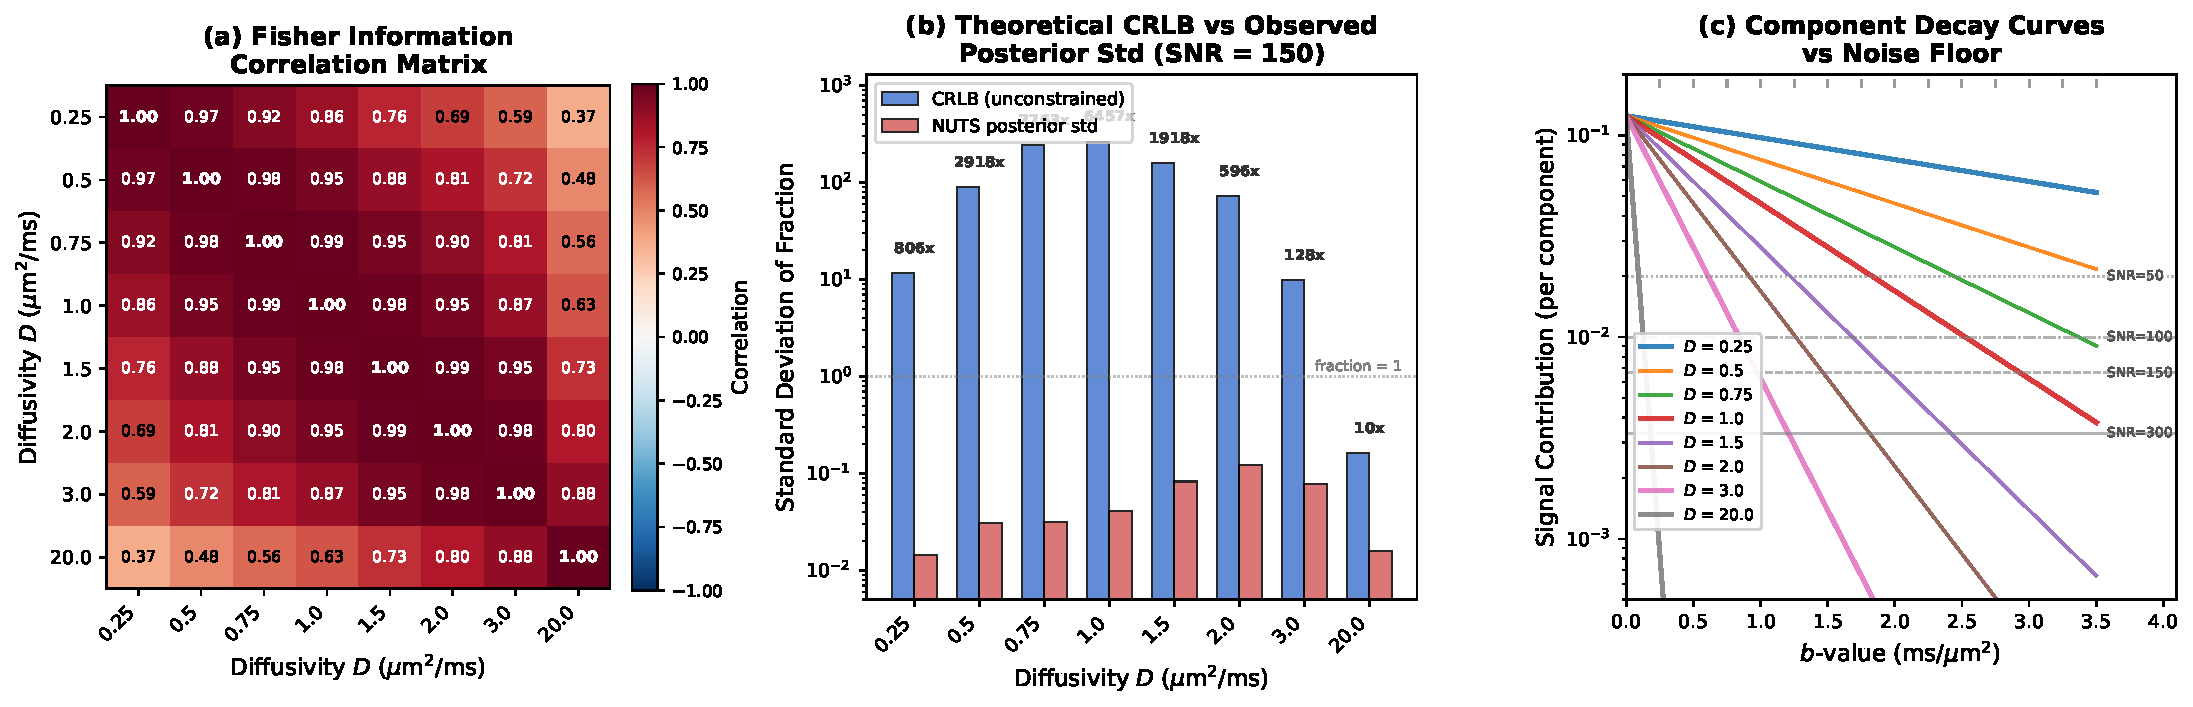
\includegraphics[width=\textwidth]{figures/fig_fisher.pdf}
\caption{%
Fisher information analysis of the spectral discretization.
(a)~Fisher information correlation matrix: adjacent diffusivity components
($D = 0.50$--$1.00\;\umsmm$) have mutual correlation $> 0.99$, making them
fundamentally indistinguishable from 15 b-value measurements.
$D = 0.25$ and $D = 20.0\;\umsmm$ are the most separable components.
(b)~Unconstrained Cram\'er-Rao lower bound (gray) versus observed NUTS
posterior standard deviation (orange) at SNR = 150.
Labels show the improvement factor.
Non-negativity constraints and Bayesian priors reduce estimation error by
100--8000$\times$, demonstrating their essential role.
(c)~Individual component decay curves $R_j \exp(-b D_j) / K$ at equal
fractions, with horizontal noise floors at SNR = 50--300.
Slow-diffusing components (e.g., $D = 0.25\;\umsmm$) contribute signal
across all b-values; fast components ($D \geq 3.0\;\umsmm$) decay below the
noise floor within the first few b-value steps, motivating the sparser
discretization at high diffusivities.
}
\label{fig:fisher}
\end{figure}
